\chapter{Función Logaritmo, función exponencial y funciones trigonométricas inversas}

\setcounter{section}{1}
\section{definición de logaritmo natural como integral}

Una ecuación tal como 
$$f(xy)=f(x)+f(y)$$ 
que expresa una relación entre los valores de una función en dos o más puntos se denomina \textbf{ecuación funcional}. Una solución de $f(xy)=f(x)+f(y)$ es la función que es cero en todo el eje real; y además es la única solución que está definida para todos los números reales. En efecto: sea $f$ una función que satisfaga la ecuación funcional, si $0$ pertenece al dominio de $f$ se puede poner $y=0$ obteniéndose $f(0)=f(x)+f(0)$ lo que implica $f(x)=0$ para cada $x$ en el dominio de $f$. Dicho de otra forma, si $0$ pertenece al dominio de $f$, $f$ ha de ser idénticamente nula. Por tanto, una solución no idénticamente nula no puede estar definida en $0$.\\

Si $f$ es una solución de $f(xy)=f(x)+f(y)$ y el dominio de $f$ contiene el punto $1$, se puede poner $x=y=1$ y se obtiene $f(1)=2f(1)$ de donde
$$f(1)=0.$$
Si ambos $1$ y $-1$ pertenecen al dominio de $f$ se puede tomar $x=-1$ e $y=-1$ de donde se deduce $f(1)=2f(-1)$ es decir $f(-1)=0$. Si ahora, $x$, $-x$, $1$, $-1$ pertenecen al dominio de $f$ se puede poner $y=-1$ obteniéndose $f(-x)=f(-1)+f(x)$, y puesto que $f(-1)=0$ se tiene
$$f(-x)=f(x).$$
Es decir, toda solución de $f(xy)=f(x)+f(y)$ es necesariamente una función par.\\

Supóngase ahora, que $f$ tiene una derivada $f'(x)$ en cada $x\neq 0$. Dejando fijo en $f(xy)=f(x)+f(y)$ y derivando con respecto a $x$ (aplicando en el primer miembro la regla de la cadena) se tiene:
$$yf'(xy)=f'(x).$$
Si $x=1$, de esta ecuación se deduce $yf'(y)=f'(1)$. Por tanto:
$$f'(y)=\dfrac{f(1)}{y}\mbox{ para cada }y\neq 0.$$

La derivada es monótona e integrable en cada intervalo cerrado que no contenga el origen. Además, $f'$ es continua en cada uno de estos intervalo y se puede aplicar el segundo teorema fundamental del cálculo:
$$f(x)-f(c)=\int_c^x f'(t)\; dt = f'(1)\int_c^x \dfrac{1}{t}\; dt.$$
Si $x>0$, esta ecuación es válida para cada positivo $c>0$, y si es $x<0$ es válida para cada $c$ negativo. Puesto que $f(1)=0$, eligiendo $c=1$ se tiene
$$f(x)=f'(1)\int_1^x \dfrac{1}{t}\; dt\quad \mbox{ si } \quad x>0.$$
Si $x$ es negativa, $-x$ es positiva y puesto que $f(x)=f(-x)$ se tiene:
$$f(x)=f'(1)\int_1^{-x}\dfrac{1}{t}\; dt\quad \mbox{si}\quad x<0.$$
Estas dos formulas se puede unir en una sola:
$$f(x)=f'(1)\int_1^{|x|}\dfrac{1}{t}\; dt\quad \mbox{si}\quad x\neq 0.$$
En consecuencia, si existe una solución de $f(xy)=f(x)+f(y)$ que tiene una derivada en cada punto $x\neq 0$ esta solución ha de venir dada necesariamente por la fórmula integral de $f(x)=f'(1)\int_1^{|x|}\frac{1}{t}\; dt$. Si $f'(1)=0$ entonces $f(x)=0$ para cada $x\neq 0$ y esta solución coincide con la idénticamente nula. Por tanto, si $f$ no es idénticamente nula ha de ser $f'(1)\neq 0$, en cuyo caso se pueden dividir ambos miembros por $f'(1)$ obteniéndose
$$g(x)=\int_1^{|x|}\dfrac{1}{t}\; dt\quad \mbox{si}\quad x\neq 0.$$
donde $g(x)=f(x)/f'(1)$. La función $g$ es también una solución de $f(xy)=f(x)-f(y)$, puesto que si $f$ es solución también lo es $cf$. Esto demuestra que si tiene una solución que no es la idénticamente nula, y si esta función es derivable en todos los puntos, excepto en el origen, entonces la función $f$ es una solución, y todas las soluciones pueden obtenerse de estar multiplicando $g$ por una constante conveniente.\\

Dos números distintos tendrían un mismo logaritmo, puesto que la función $g$ tendría la propiedad: $g(x) = g( - x)$. En atención a consideraciones que posteriormente se harán, es preferible definir el logaritmo de manera que dos números distintos no tengan el  mismo logaritmo, lo cual se logra definiendo el logaritmo sólo para los números positivos. Por tanto, se tomará la siguiente definición.


\section{Definición de logaritmo. Propiedades fundamentales}

%-------------------- Definición de logaritmo  6.1.
\begin{def.}
    Si $x$ es un número real positivo, definamos el logaritmo natural de $x$, designando provisionalmente por $L(x)$, como la integral
    $$L(x)=\int_1^{x}\dfrac{1}{t}\; dt.$$
    Cuando $x>1$, $L(x)$ puede interpretarse geométricamente como el área de la región sombreada.
\end{def.}

%-------------------- Teorema 6.1.
\begin{teo}
    La función logaritmo tiene las propiedades siguientes:
    \begin{enumerate}[a)]
	\item $L(1)=0.$
	\item $L'(x)=\dfrac{1}{x}$ para todo $x>0.$
	\item $L(ab)=L(a)+L(b)$ para todo $a>0$, $b>0.$\\
    \end{enumerate}
	Demostración.-\; La parte a) se deduce inmediatamente de la definición. Para demostrar b), observamos simplemente que $L$ es una integral indefinida de una función continua y apliquemos el primer teorema fundamental del Cálculo. La propiedad c) es consecuencia de la propiedad aditiva de la integral. Escribamos
	$$L(ab)=\int_1^{ab}\dfrac{dt}{t}=\int_1^a \dfrac{dt}{t}+\int_a^{ab}\dfrac{dt}{t}=L(a)+\int_a^{ab}\dfrac{dt}{t}.$$
	En la última integral hemos hecho la sustitución $u=t/a$, $du=dt/a$, y encontramos que la integral se deduce a $L(b)$, lo que demuestra c).
\end{teo}


\section{Gráfica del logaritmo natural}
La derivada segunda es $L''(x) = - 1/x^2$ que es negativa para todo $x$, por lo que $L$ es una función cóncava.

\section{Consecuencias de la ecuación funcional \boldmath$L(ab)=L(a)+L(b)$}

La función no está acotada superiormente; esto es, para todo número positivo $M$ (por grande que sea) existen valores de $x$ tales que
$$L(x)>M.$$
Podemos deducirlo de la ecuación funcional. Cuando $a=b$, tenemos $L\left(a^2\right)=2L(a)$. Utilizando la ecuación funcional una vez más poniendo $b=a^2$, obtenemos $L\left(a^3\right)=3L(a)$. Por inducción encontramos la fórmula general
$$L\left(a^n\right)=nL(a)$$
para cualquier entero $n\geq 1$. Cuando $a=2$, se obtiene $L\left(2^n\right)=nL(2)$, y por tanto resulta
$$L\left(2^n\right) \quad \mbox{cuando}\quad n>\dfrac{M}{L(2)}.$$
Esto demuestra la afirmación 
$$L(x)>M.$$
Tomando $b=1/a$ en la ecuación funcional, encontramos $L(1/a)=-L(a)$. En particular, cuando $a=2^n$, habiendo elegido $n$ como en $L(x)>M$, se tiene
$$L\left(\dfrac{1}{2^n}\right)=-L(2^n)<-M,$$
lo que indica que tampoco existe cota inferior para los valores de la función.

%-------------------- Teorema 6.2.
\begin{teo}
    Para cada número real $b$ existe exactamente un número real positivo $x$ cuyo logaritmo, $L(a)$, es igual a $b$.\\\\
    Demostración.-\; Si $b>0$, elegimos un entero cualquiera $n>b/L(2)$. Entonces, en virtud de $L(x)>M$, $L\left(2^n\right)>b.$ Seguidamente examinamos la función $L$ en el intervalo cerrado $[1,2^n]$. Su valor en el extremo izquierdo es $L(1)=0$, y en el extremo derecho es $L(2^n)$. Puesto que $0<b<L\left(2^n\right)$, el teorema del valor intermedio para funciones continuas (teorema 3.8, sección 3.10) asegura la existencia por lo menos de un $a$ tal que $L(a)=b$. No puede existir otro valor $a'$ tal que $L\left(a'\right)=b$ porque esto significaría $L(a)=L\left(a'\right)$ para $a\neq a'$, y esto contradice la propiedad de crecimiento del logaritmo. Por consiguiente la proposición $L(a)=b$ ha sido demostrada para $b>0$. La demostración para $b$ negativo es consecuencia de esa si utilizamos la igualdad $L(1/a)=-L(a)$.
\end{teo}

En particular, existe un único número cuyo logaritmo natural es igual a $1$. Este número, al igual que $\pi$, se encuentra tan repetidamente en fórmulas matemáticas que es inevitable el adoptar para él un símbolo especial. Este número es $e$.

%-------------------- Definición 6.2.
\begin{def.}
    Designamos por $e$ el número para el que
    $$L(e)=1.$$
\end{def.}

Los logaritmos naturales se denomina también \textbf{logaritmos neperianos}. En honor al inventor, Juan Neper (1550-1617). Es frecuente en la práctica utilizar los símbolos $\ln x$ o $\log x$ en vez de $L(x)$ para designar el logaritmo de $x$.


\section{Logaritmos referidos a un base positiva \boldmath $b\neq 1$}

En la sección 6.2 se vio que la función $f$ más general derivable en el eje real, que satisface la ecuación funcional $f(xy)=f(x)+f(y)$ está por la fórmula
$$f(x)=c\log x,$$
donde $c$ es una constante. Para cada $c$ esta $f(x)$ se denominará el logaritmo de $x$ asociado a $c$, y como es evidente, su valor no será necesariamente el mismo que el logaritmo natural de $x$. Si $c=0$, $f$ es idénticamente nulo y este caso carece de interés. Si $c\neq 0$ se indicará de otra forma la dependencia de $f$ y $c$ introduciendo el concepto de \textbf{base} de logaritmos.\\
De $f(x)=c\log x$ se deduce que cuando $c\neq 0$ existe un número real único $b>0$ tal que $f(b)=1$. Esta $b$ está relacionada con $c$ por medio de la igualdad $c\log b=1$; como $b\neq 1$ es $c=1/\log b,$ lo que expresamos como
$$f(x)=\dfrac{\log x}{\log b}.$$

Para esta elección de $c$ se dice que $f(x)$ es el logaritmo de $x$ en base $b$ y se escribe $\log_b x$ en vez de $f(x)$.

%-------------------- Definición 6.3.
\begin{def.}
    Si $b>0$, $b\neq 1$, y si $x>0$, el logaritmo de $x$ en base $b$ es el número
    $$\log_b x = \dfrac{\log x}{\log b},$$
    donde los logaritmos del segundo miembro son logaritmos naturales.
\end{def.}

Obsérvese que $\log_b b = 1$. Si $b=e$ se tiene $\log_e x= \log x$, es decir, los logaritmos naturales son los que tienen de base $e$. Puesto que los logaritmos de base $e$ son los más frecuentemente usando en matemáticas, la palabra logaritmo indica casi siempre el logaritmo natural.


\section{Fórmulas de derivación e integración en las que intervienen logaritmos}
Puesto que la derivada del logaritmo viene dada por la fórmula $D\log x = 1/x$ para $x>0$, se tiene la fórmula de integración 
$$\int \dfrac{1}{x}\; dx = \log(x)+C.$$
Aún más general, si $u=f(x)$, siendo $f$ una función con derivada continua, se tiene
$$\int \dfrac{du}{u} = \log u + C \quad \mbox{o}\quad \int \dfrac{f'(x)}{f(x)}\; dx = \log f(x) + C.$$
para $u$ o $f(x)$ positiva.\\

Afortunadamente, es fácil extender el campo de validez de etas fórmulas de manera que pueden aplicarse para funciones que sean positivas o negativas, pero no cero. Se introduce simplemente una nueva función $L_0$ definida para todos los números reales $x\neq 0$ por la ecuación:
$$L_0(x)=\log|x|=\int_1^{|x|}\dfrac{1}{t}\; dt.$$
Puesto que $\log|xy|=\log(|x||y|)=\log|x|+\log|y|$, la función $L_0$ satisface también la ecuación funcional básica; es decir, se tiene:
$$L_0(xy)=L_0(x)+L_0(y)$$
para $x$ e $y$ reales cualesquiera distintos de cero. Para $x>0$ se tiene $L_0'(x)=1/x$ ya que $L_0(x)$ para $x$ positivo es lo mismo que $\log(x)$. La fórmula de la derivada vale también para $x<0$ puesto que en este caso $L_0(x)=L(-x)$ y por tanto $L_0(x)=-L'(-x)=-1/(-x)=1/x$. De aquí resulta
$$L_0'(x)=\dfrac{1}{x}\quad \mbox{para todo valor real }\; x\neq 0.$$
Por tanto, si en las fórmulas de integración precedentes se pone $L_0$ en vez de $L$, se puede extender su alcance a funciones que toman valores tanto negativos como positivos. Por ejemplo 
$$\int \dfrac{du}{u} = \log u + C \quad \mbox{o}\quad \int \dfrac{f'(x)}{f(x)}\; dx = \log f(x) + C.$$
se puede generalizar como sigue:
$$\int \dfrac{du}{u} = \log |u| + C, \quad \int \dfrac{f'(x)}{f(x)}\; dx = \log |f(x)| + C.$$
Evidentemente, cuando se aplique junto con el segundo teorema funda- mental del Cálculo para calcular una integral indefinida no se pueden tomar intervalos que incluyan puntos en los que $u$ o $f(x)$ sean cero.


Una de las propiedades más notables de la función exponencial es la fórmula
$$E'(x)=E(x),$$
que nos dice que la función es su propia derivada. \\

Supongamos $f(x)=a^x$ para $x>0$. Según la definición de $a^x$, podemos escribir
$$f(x)=e^{x\log a}=E(x\log a);$$
luego en virtud de la regla de cadena, encontramos
$$f'(x)=E'(x\log a )\cdot \log a=E(x\log a)\cdot \log a=a^x\log a.$$
Dicho de otro modo, la derivación de $a^x$ multiplica simplemente $a^x$ por el factor constante $\log a$, siendo este factor $1$ cuando $a=e$. Por ejemplo $E'(x)=E(x)$ da como resultado 
$$\int e^x \; dx = e^x+C,$$
en tanto que $f'(x)=a^x\log a$ conduce a la fórmula más general
$$\int a^x \; dx = \dfrac{a^x}{\log a}+C \quad (a>0,\; a\neq 1).$$
Sustituimos $x$ en $\int e^x \; dx = e^x+C,$ y la ecuación anterior por $u$ obteniendo
$$\int e^u \; du = e^u+C, \quad \int a^u \; du = \dfrac{a^u}{\log a}+C (a>0,\; a\neq 1),$$
donde $u$ representa cualquier función con derivada continua. Si escribimos $u=f(x),$ y $fu=f'(x)\; dx$, las fórmulas anteriores se convierten En
$$\int e^{f(x)} f'(x) \; dx = e^{f(x)}+C, \quad \int a^{f(x)} f'(x) \; dx = \dfrac{a^{f(x)}}{\log a}+C (a>0,$$
siendo la segunda integral válida para $a>0$, $a\neq 1$.

%-------------------- Ejercicio 6.1
\begin{ejem}
    Integrar $\displaystyle\int x^2e^{x^3}\;dx.$\\\\
	Respuesta.-\; Sea $u=x^3$. Entonces, $fu=3x^2\; dx$  y se obtiene
	$$\int x^2e^{x^3}\; dx = \dfrac{1}{3}\int e^{x^3}(3x^2\; dx)=\dfrac{1}{3}\int e^u\; dx = \dfrac{1}{3}e^{x^3}+C.$$
\end{ejem}

%-------------------- Ejercicio 6.2
\begin{ejem}
    Integrar $\displaystyle\int \log(x)\; dx.$\\\\
	Respuestas.-\; Sea $u=\log(x)$, $dv=dx.$ Entonces, $du=dx/x$, $v=x$, y obtenemos
	$$\int \log(x)\; dx = \int u\; dv = uv-\int v\; du = x\log(x)-\int x\dfrac{1}{x}\; dx = x\log(x)-x+C.$$
\end{ejem}


\section{Derivación logarítmica}
El método fue desarrollado en 1697 por Johann Bernoulli (1667-1748) y su fundamento es una hábil aplicación de la regla de la cadena.\\

Supóngase que se forma la función compuesta de $L_0$ con una función derivable cualquier $f(x)$; es decir,
$$g(x)=L_0\left[f(x)\right] = \log|f(x)|$$
para todo $x$ tal que $f(x)\neq 0$. La regla de la cadena aplica junto con $L'_0(x)=\dfrac{1}{x},\; x\neq 0$ conduce a la fórmula
$$g'(x)=L'_0\left[f(x)\right]\cdot f'(x)=\dfrac{f'(x)}{f(x)}.$$
Si la derivada $f'(x)$ se puede calcular de otra forma, entonces se puede obtener $f'(x)=g¡(x)\cdot f(x)$.

%-------------------- Ejercicio 6.2.
\begin{ejem}
    Calcular $f'(x)$ si $f(x)=x^2\cos x\left(1+x^4\right)^{-7}.$\\\\
	Respuesta.-\; Se toma el logaritmo del valor absoluto de $f(x)$ y luego se deriva.\\
	Sea pues
	$$
	\begin{array}{rcl}
	    g(x)&=&\log|f(x)|\\
		&=&\log x^2 + \log|\cos x| + \log\left(1+x^4\right)^{-7}\\
		&=& 2\log x + \log|\cos x| - 7\log\left(1+x^4\right)
	\end{array}
	$$
	Derivando $g(x)$ con respecto a $x$ se obtiene
	$$
	\begin{array}{rcl}
	    g'(x) &=& \dfrac{f'(x)}{f(x)}\\\\
		  &=& \dfrac{2}{x}-\dfrac{\sen x}{\cos x}-\dfrac{28x^3}{(1+x^4)}.
	\end{array}
	$$
	Multiplicando ambos miembros por $f(x)$ tenemos
	$$
	\begin{array}{rcl}
	    f'(x) &=& \dfrac{2x\cos x}{\left(1+x^4\right)^7}-\dfrac{x^2\sen x}{\left(1+x^4\right)^7}-\dfrac{28x^5}{\left(1+x^4\right)^7}
	\end{array}
	$$

\end{ejem}


\section{Ejercicios}

\begin{enumerate}[\bfseries 1.]

    %-------------------- 1.
    \item 
	\begin{enumerate}[a)]

	    %---------- a)
	    \item Hallar todos los valores de $c$ tales que $\log x = c + \displaystyle\int_e^x t^{-1}\; dt$ para todo $x>0$.\\\\
		Respuesta.- Resolvamos de la siguiente manera:
		$$
		\begin{array}{rcl}
		    \log(x) = c+\displaystyle\int_c^x \dfrac{1}{t}\; dt &\Rightarrow& \log(x) = c+\log(x)-\log(c)\\\\
									&\Rightarrow& \log(x)=c+\log(x)-1\\\\ 
									&\Rightarrow& c=1.
		\end{array}
		$$

	    %---------- b)
	    \item Sea $f(x)=\log\left[(1+x)/(1-x)\right]$ si $x>0$. Si $a$ y $b$ son números dados, siendo $ab\neq -1$, hallar todos los $x$ tales que $f(x)=f(a)+f(b)$.\\\\
		Respuesta.- Resolvamos de la siguiente manera:
		$$
		\begin{array}{rcl}
		    f(x)=f(a)+f(b) &\Rightarrow& \log\left(\dfrac{1+x}{1-x}\right) = \log\left(\dfrac{1+a}{1-a}\right)+\log\left(\dfrac{1+b}{1-b}\right)\\\\
				   &\Rightarrow& \log\left(\dfrac{1+x}{1-x}\right) = \log\left[\dfrac{(1+a)(1+b)}{(1-a)(1-b)}\right]\\\\
				   &\Rightarrow& \dfrac{1+x}{1-x} = \dfrac{(1+a)(1+b)}{(1-a)(1-b)}\\\\
				   &\Rightarrow& x = \dfrac{a+b}{1+ab}.
		\end{array}
		$$
		\vspace{.5cm}

	\end{enumerate}

    %-------------------- 2.
    \item En cada caso, hallar un $x$ real que satisfaga la igualdad dada,

	\begin{enumerate}[(a)]

	    %---------- a)
	    \item $\log(1+x)=\log(1-x)$.\\\\
		Respuesta.-\; Calculemos de la siguiente manera:
		$$
		\begin{array}{rcl}
		    \log(1+x)=\log(1-x) &\Rightarrow& 1+x=1-x\\\\
					&\Rightarrow& x=0.
		\end{array}
		$$
		\vspace{.5cm}

	    %---------- b)
	    \item $\log(1+x)=1+\log(1-x)$.\\\\
		Respuesta.-\; Calculemos de la siguiente manera:
		$$
		\begin{array}{rcl}
		    \log(1+x)=1+\log(1-x) &\Rightarrow& \log\left(\dfrac{1+x}{1-x}\right)=1\\\\
					  &\Rightarrow& \dfrac{1+x}{1-x}=e\\\\
					  &\Rightarrow& x=\dfrac{e-1}{e+1}.
		\end{array}
		$$
		\vspace{.5cm}

	    %---------- c)
	    \item $2\log(x) = x\log(2), \; x\neq 2$.\\\\
		Respuesta.-\; Calculemos de la siguiente manera:
		$$
		\begin{array}{rcl}
		    2\log(x) = x\log(2), \; x\neq 2 &\Rightarrow& \log(x^2)=\log(2^x)\\\\
						     &\Rightarrow& x^2=2^x\\\\
						     &\Rightarrow& x=2,\; x=4.
		\end{array}
		$$
		\vspace{.5cm}

	    %---------- d)
	    \item $\log\left(\sqrt{x}+\sqrt{x+1}\right)=1$.\\\\
		Respuesta.-\; Calculemos de la siguiente manera:
		$$
		\begin{array}{rcl}
		    \log\left(\sqrt{x}+\sqrt{x+1}\right)=1 &\Rightarrow& \sqrt{x}+\sqrt{x+1}=e\\\\
							   &\Rightarrow& x-(x+1)=e\left(\sqrt{x}-\sqrt{x+1}\right)\\\\
							   &\Rightarrow& \sqrt{x+1}-\sqrt{x}=\dfrac{1}{e}\\\\
							   &\Rightarrow& \left(\sqrt{x+1}-\sqrt{x}\right)+\left(\sqrt{x+1}-\sqrt{x}\right)=\dfrac{1}{e}+e\\\\
							   &\Rightarrow& 2\sqrt{x+1}=e+\dfrac{1}{e}\\\\
							   &\Rightarrow& \sqrt{x+1}=\dfrac{e}{2}+\dfrac{1}{2e}\\\\
							   &\Rightarrow& x+1=\dfrac{e^2}{4}+\dfrac{1}{4e^2}+\dfrac{1}{2}\\\\
							   &\Rightarrow& x=\dfrac{\left(e^2-1\right)^2}{4x^2}.
		\end{array}
		$$
		\vspace{.5cm}

	\end{enumerate}

    %-------------------- 3.
    \item Sea $f(x)=\frac{\log(x)}{x}$. Describir los intervalos en los que $f$ es creciente, decreciente, convexa y cóncava. Esbozar la gráfica de $f$.\\\\
	Respuesta.-\; Tomemos primero la segunda derivada de $f$:
	$$
	\begin{array}{rcl}
	    f(x) &=& \dfrac{\log(x)}{x}\\\\
	    f'(x) &=& \dfrac{1-\log(x)}{x^2}\\\\
	    f''(x) &=& \dfrac{2\log(x)-3}{x^3}.
	\end{array}
	$$
	Se sigue que,
	$$
	\left\{
	\begin{array}{rcl}
	    f'(x)>0 &\mbox{para} & 0<x<e\\\\
	    f'(x)<0 &\mbox{para} & x>e.
	\end{array}
	\right.
	$$

	Esto significa que $f$ es es creciente en $0<x<e$ y decreciente en $x>e$.\\
	
	Luego se tiene, 
	$$
	\left\{
	\begin{array}{rcl}
	    f''(x)<0 &\mbox{para} & 0<x<\sqrt{e^3}\\\\
	    f''(x)>0 &\mbox{para} & x>\sqrt{e^3}.
	\end{array}
	\right.
	$$
	Lo que significa que $f$ es cóncava en $0<x<\sqrt{e^3}$ y convexa en $x>\sqrt{e^3}$.
	\begin{center}
	    \begin{tikzpicture}
		\begin{axis}[scale=.5,draw opacity =.5,samples=100,smooth, 
		  axis x line=center, 
		  axis y line=center,
		  ylabel = {$f(x)$},
		  xlabel = {$x$},
		  xlabel style={below right},
		  ylabel style={above left},
		  label style={font=\tiny},
		  tick label style={font=\tiny},
		  enlargelimits=upper] 
		  \addplot[black,opacity=1,domain=0.7:5]{ln(x)/x};
		\end{axis}
	    \end{tikzpicture}
	\end{center}
	\vspace{.5cm}

    \end{enumerate}

    En los ejercicios 4 al 14, hallar la derivada $f'(x)$. En cada caso, la función $f$ se supone definida para todo $x$ real para los que la fórmula dada para $f(x)$ tiene sentido.\\

\begin{enumerate}[\bfseries 1.]
\setcounter{enumi}{3}

    %-------------------- 4.
    \item $f(x)=\log\left(1+x^2\right)$.\\\\
	Respuesta.-\; Usando la regla de la cadena tenemos que,
	$$f'(x)= \dfrac{1}{1+x^2}\cdot 2x =\dfrac{2x}{1+x^2}.$$\\

    %-------------------- 5.
    \item $f(x)=\log\left(\sqrt{1+x^2}\right)$.\\\\
	Respuesta.-\; Usando la regla de la cadena tenemos que,
	$$f'(x)= \left(\dfrac{1}{\sqrt{1+x^2}}\right)\left( \dfrac{1}{2\sqrt{1+x^2}}\right)(2x) =\dfrac{x}{1+x^2}.$$\\

    %-------------------- 6.
    \item $f(x)=\log\left(\sqrt{4-x^2}\right)$.\\\\
	Respuesta.-\; Usando la regla de la cadena tenemos que,
	$$f'(x)= \left(\dfrac{1}{\sqrt{4-x^2}}\right)\left( \dfrac{1}{2\sqrt{4-x^2}}\right)(-2x) =\dfrac{x}{x^2-4}.$$\\

    %-------------------- 7.
    \item $f(x)=\log\left(\log(x)\right)$.\\\\
	Respuesta.-\; Usando la regla de la cadena tenemos que,
	$$f'(x)= \dfrac{1}{\log(x)}\cdot \dfrac{1}{x} =\dfrac{1}{x\log(x)}.$$\\

    %-------------------- 8.
    \item $f(x)=\log\left(x^2 \log(x)\right)$.\\\\
	Respuesta.-\; Usando la regla de la cadena y la regla del producto tenemos que,
	$$f'(x)= \left[\dfrac{1}{x^2\log(x)}\right]\left[2x\log(x) + x\right] =\dfrac{1}{x^2\log(x)}\cdot 2x\log(x)+\dfrac{1}{x\log(x)} =\dfrac{2}{x}+\dfrac{1}{x\log(x)}.$$\\

    %-------------------- 9.
    \item $f(x)=\dfrac{1}{4}\log\left(\dfrac{x^2-1}{x^2+1}\right)$.\\\\
	Respuesta.-\; Usando la regla de la cadena y la regla del cociente tenemos que,
	$$
	\begin{array}{rcl}
	    f'(x)&=&\dfrac{1}{4}\left(\dfrac{2x}{x^2-1}-\dfrac{2x}{x^2+1}\right)\\\\
		 &=& \dfrac{1}{4}\left[\dfrac{2x(x^2+1)-2x(x^2-1)}{(x^2-1)(x^2+1)}\right]\\\\
		 &=& \dfrac{1}{4}\left[\dfrac{2x^3+2x-2x^3+2x}{(x^2-1)(x^2+1)}\right]\\\\
		 &=& \dfrac{x}{x^4-1}.
	\end{array}
	$$
	\vspace{.5cm}

    %-------------------- 10.
    \item $f(x)=(x+\sqrt{1+x^2})^n$.\\\\
	Respuesta.-\; Tomando el logaritmo del valor absoluto de la función dada tenemos que,
	$$
	\begin{array}{rcl}
	    g(x) &=& \log|f(x)|\\\\
		 &=& |n|\log\left| (x+\sqrt{1+x^2})\right|.
	\end{array}
	$$
	Derivando $g'(x)$,
	$$
	\begin{array}{rcl}
	    g'(x) &=& \dfrac{f'(x)}{f(x)}\\\\
		  &=& n\left(\dfrac{1}{x+\sqrt{1+x^2}}\right)\left(1+\dfrac{x}{\sqrt{1+x^2}}\right)\\\\
		  &=& \dfrac{n}{\sqrt{1+x^2}}.
	\end{array}
	$$

	Ahora, multiplicando $g'(x)$ por $f(x)$ tenemos que,
	$$
	\begin{array}{rcl}
	    f(x)\cdot \dfrac{f'(x)}{f(x)} &=& \dfrac{n}{\sqrt{1+x^2}}\cdot \left(x+\sqrt{1+x^2}\right)^n\\\\
	    f'(x) &=& \dfrac{n\left(x+\sqrt{1+x^2}\right)^n}{\sqrt{1+x^2}}.
	\end{array}
	$$
	\vspace{.5cm}

    %-------------------- 11.
    \item $f(x)=\sqrt{x+1}-\log(1+\sqrt{x+1})$.\\\\
	Respuesta.-\; Usando la regla de la cadena,
	$$	
	\begin{array}{rcl}
	    f'(x) &=& \dfrac{1}{2\sqrt{x+1}}-\dfrac{1}{1+\sqrt{x+1}}\cdot \dfrac{1}{2\sqrt{x+1}}\\\\
		  &=& \dfrac{1}{2\sqrt{x+1}}\left(1-\dfrac{1}{1+\sqrt{x+1}}\right)\\\\
		  &=& \dfrac{1}{2\left(1+\sqrt{x+1}\right)}.
	\end{array}
	$$
	\vspace{.5cm}


    %-------------------- 12.
    \item $f(x)=x\log\left(x+\sqrt{1+x^2}\right)-\sqrt{1+x^2}$.\\\\
	Respuesta.-\; Usnaod la regla de la cadena y la regla del producto tenemos que,
	$$
	\begin{array}{rcl}
	    f'(x) &=& \log\left(x+\sqrt{1+x^2}\right)+\left(\dfrac{x}{x+\sqrt{1+x^2}}\right)\left(1+\dfrac{x}{\sqrt{1+x^2}}\right)-\dfrac{x}{\sqrt{1+x^2}}\\\\
		  &=& \log\left(x+\sqrt{1+x^2}\right)+\dfrac{x}{\sqrt{1+x^2}}-\dfrac{x}{\sqrt{1+x^2}}\\\\
		  &=& \log\left(x+\sqrt{1+x^2}\right).
	\end{array}
	$$
	\vspace{.5cm}

    %-------------------- 13.
    \item $f(x)=\dfrac{1}{2\sqrt{ab}}\log\left(\dfrac{\sqrt{a}+x\sqrt{b}}{\sqrt{a}-x\sqrt{b}}\right)$.\\\\
	Respuesta.-\; Usando la regla de la cadena y la regla del cociente tenemos que,
	$$
	\begin{array}{rcl}
	    f'(x) &=& \dfrac{1}{2\sqrt{ab}}\left(\dfrac{\sqrt{a}-x\sqrt{b}}{\sqrt{a}+x\sqrt{b}}\right)\left[\dfrac{\sqrt{b}\left(\sqrt{a}-x\sqrt{b}\right)+\sqrt{b}\left(\sqrt{a}+x\sqrt{b}\right)}{\left(\sqrt{a}-x\sqrt{b}\right)^2}\right]\\\\
		  &=& \dfrac{1}{2\sqrt{ab}}\cdot \dfrac{2\sqrt{ab}}{\left(\sqrt{a}+x\sqrt{b}\right)\left(\sqrt{a}-x\sqrt{b}\right)}\\\\
		  &=& \dfrac{1}{a^2-bx^2}.
	\end{array}
	$$
	\vspace{.5cm}

    %-------------------- 14.
    \item $f(x)=x\left[\sen(\log x)-\cos(\log x)\right]$.\\\\
	Respuesta.-\; Usando la regla de la cadena y la regla del producto tenemos que,
	$$
	\begin{array}{rcl}
	    f'(x) &=& \left[\sen(\log x)-\cos(\log x)\right]+x\left[\dfrac{\cos(\log x)}{x}+\dfrac{\sen(\log x)}{x}\right]\\\\
		  &=& 2\sen(\log x).
	\end{array}
	$$
	\vspace{.5cm}

    %-------------------- 15.
    \item $f(x)=\log_xe$.\\\\
	Respuesta.-\; Por definición de logaritmo en base $x$ tenemos que,
	$$f(x)=\log_xe=\dfrac{\log e}{\log x}.$$
	De donde, el logaritmo de $e$ es la constante $1$, por lo tanto
	$$f(x)=\dfrac{1}{\log x}.$$
	Luego, usando la regla del cociente tenemos que,
	$$	
	\begin{array}{rcl}
	    f'(x) &=& \dfrac{-\dfrac{1}{x}}{\left(\log x\right)^2}\\\\
		  &=& -\dfrac{1}{x\left(\log x\right)^2}.
	\end{array}
	$$
	\vspace{.5cm}

\end{enumerate}

En los ejercicios 16 al 26, calcular las integrales.\\

\begin{enumerate}[\bfseries 1.]
\setcounter{enumi}{15}

    %-------------------- 16.
    \item $\displaystyle\int \dfrac{dx}{2+3x}$.\\\\
	Respuesta.-\; 
	$$\int \dfrac{1}{2+3x}\; dx = \dfrac{1}{3}\int \dfrac{3}{2+3x}\; dx=\dfrac{1}{3}\log|2+3x|+C.$$\\

    %-------------------- 17.
    \item $\displaystyle\int \log^2(x)\; dx$.\\\\
	Respuesta.-\; Usando la integración por partes,
	$$
	\begin{array}{rcl}
	    u=\left(\log|x|\right)^2 &\Rightarrow& du=\dfrac{2\log(x)}{x}\; dx\\\\
	    dv=dx &\Rightarrow& v=x.
	\end{array}
	$$
	Notemos por el ejemplo 6.2 de, 
	$$\int \log(x)\; dx = x\log|x|-x+C.$$
	Por lo tanto,
	$$
	\begin{array}{rcl}
	    \displaystyle\int (\log x)^2\; dx &=& \displaystyle\int u\; dv\\\\
					      &=& uv - \displaystyle\int v\; du\\\\
					      &=& x(\log|x|)^2-\displaystyle\int 2\log x \; dx\\\\
					      &=& x(\log|x|)^2 - 2(x\log|x|-x)+C\\\\
					      &=& x(\log|x|)^2-2x\log|x|+2x+c.
	\end{array}
	$$
	\vspace{.5cm}

    %-------------------- 18.
    \item $\displaystyle\int x\log(x)\; dx$.\\\\
	Respuesta.-\; Usando la integración por partes,
	$$
	\begin{array}{rcl}
	    u=\log|x| &\Rightarrow& du=\dfrac{1}{x}\; dx\\\\
	    dv=x\;dx &\Rightarrow& v=\dfrac{x^2}{2}.
	\end{array}
	$$
	Por lo tanto,
	$$
	\begin{array}{rcl}
	    \displaystyle\int x\log x \; dx &=& \displaystyle\int u\; dv\\\\
					    &=& uv-\displaystyle v\; du\\\\
					    &=& \dfrac{1}{2}x^2\log|x|-\dfrac{1}{2}\displaystyle\int x\; dx\\\\
					    &=& \dfrac{1}{2}x^2\log|x|-\dfrac{1}{4}x^2+C.
	\end{array}
	$$
	\vspace{.5cm}

    %-------------------- 19.
    \item $\displaystyle\int x\log^2(x)\; dx$.\\\\
	Respuesta.-\; Usando la integración por partes,
	$$
	\begin{array}{rcl}
	    u=\log^2(x) &\Rightarrow& du=\dfrac{2\log(x)}{x}\; dx\\\\
	    dv=x\; dx &\Rightarrow& v=\dfrac{x^2}{2}.
	\end{array}
	$$
	Entonces,
	$$
	\begin{array}{rcl}
	    \displaystyle\int x\log^2(x) &=& \displaystyle\int u \; dv\\\\
					 &=& uv-\displaystyle\int v\; du\\\\
					 &=& \dfrac{1}{2}x^2\log^2(x)-\displaystyle\int x\log(x)\; dx.
	\end{array}
	$$
	Por el ejercicio anterior,
	$$\displaystyle\int x\log(x)\; dx = \dfrac{1}{x^2}\log|x|-\dfrac{1}{4}x^2+C.$$
	Por lo tanto,
	$$
	\begin{array}{rcl}
	    \displaystyle\int x\log^2(x)\; dx &=&  \dfrac{1}{2}x^2\log^2(x)-\displaystyle\int x\log(x)\; dx\\\\
					      &=& \dfrac{1}{2}x^2\log^2(x)-\left(\dfrac{1}{x^2}\log|x|-\dfrac{1}{4}x^2\right)+C.
	\end{array}
	$$
	\vspace{.5cm}


    %-------------------- 20.
    \item $\displaystyle\int_0^{e^3-1} \dfrac{dt}{1+t}$.\\\\
	Respuesta.-\; Usando la integración por partes,
	$$
	\begin{array}{rcl}
	    u=1+t &\Rightarrow& du=dt.\\\\
	\end{array}
	$$

	Entonces,

	$$
	\begin{array}{rcl}
	    \displaystyle\int_0^{e^3-1}\dfrac{1}{1+t}\; dt&=&\displaystyle\int_0^{e^3-1}\dfrac{1}{u}\; dt.\\\\
	\end{array}
	$$

	Ahora, ajustaremos los límites integrales calculando el límite de la función en $t=0$ y $t=e^3-1$.

	$$
	\begin{array}{rcl}
	    u &=& 1+t\\
	      &=& 1+0\\
	      &=&1.
	\end{array}
	$$

	\begin{center}
	y
	\end{center}

	$$
	\begin{array}{rcl}
	    u&=&1+t\\
	    &=&1+e^3-1\\
	    &=&e^3.
	\end{array}
	$$

	Por lo tanto,

	$$
	\begin{array}{rcl}
	    \displaystyle\int_0^{e^3-1}\dfrac{1}{1+t}\; dt&=&\displaystyle\int_1^{e^3}\dfrac{1}{u}\; du\\\\
							  &=&\left[\log(|u|)\right]\bigg|_0^{e^3}\\\\
							   &=&\left[\log(|1+t|)\right]\bigg|_0^{e^3}\\\\
							   &=&\log\left(|e^3|\right)-\log\left(|1|\right)\\\\
							   &=&3\log\left(|e|\right)\\\\
							   &=&3.
	\end{array}
	$$
	\vspace{.5cm}


    %-------------------- 21.
    \item $\displaystyle\int \cot(x)\; dx$.\\\\
	Respuesta.-\; Reescribiendo la integral se tiene,
	$$\int \cot x \; dx = \int \dfrac{\cos x}{\sen x}\; dx.$$
	Luego, usando la sustitución $u=\sen x$ y $du=\cos x\; dx$. Entonces,
	$$
	\begin{array}{rcl}
	    \displaystyle\int \cot x \; dx &=& \displaystyle\int \dfrac{\cos x}{\sen x}\; dx\\\\
					   &=& \displaystyle\int \dfrac{1}{u}\; du\\\\
					   &=& \log|u|+C\\\\
					   &=& \log|\sen x|+C.
	\end{array}
	$$
	\vspace{.5cm}

    %-------------------- 22.
    \item $\displaystyle\int x^n \log(ax)\; dx$.\\\\
	Respuesta.-\; Usando la integración por partes,
	$$
	\begin{array}{rcl}
	    u=\log(ax) &\Rightarrow& du=\dfrac{1}{x}\; dx\\\\
	    dv=x^n\; dx &\Rightarrow& v=\dfrac{x^{n+1}}{n+1}, \; si \; n\neq -1.
	\end{array}
	$$
	Entonces,
	$$
	\begin{array}{rcl}
	    \displaystyle\int x^n \log(ax)\; dx &=& \int u \; dv\\\\
						&=& uv-\displaystyle\int v\; du\\\\
						&=& \dfrac{x^{n-1}}{n+1}\log|ax| - \dfrac{1}{n+1}\displaystyle\int x^{n}\; dx\\\\
						&=& \dfrac{x^{n-1}}{n+1}\log|ax| - \dfrac{x^{n+1}}{(n+1)^2}+C.
	\end{array}
	$$

	Ahora para el caso de $n=-1$ se tiene

	$$\int x^n\log(ax)\; dx = \int \dfrac{\log(ax)}{x}\; dx.$$

	Ya que, $\frac{1}{x}\; dx$ es la derivada de $\log(ax)$, podemos sustituir $u=\log(ax)$ y $du=\frac{1}{x}\; dx$. Por lo que,

	$$
	\begin{array}{rcl}
	    \displaystyle\int \dfrac{\log(ax)}{x}\: dx &=& \displaystyle\int u\; du\\\\
						 &=& \dfrac{u^2}{2}+C\\\\
						 &=& \dfrac{(\log|ax|)^2}{2}+C.
	\end{array}
	$$
	\vspace{.5cm}


    %-------------------- 23.
    \item $\displaystyle\int x^2\log^2(x)\; dx$.\\\\
	Respuesta.-\; Usando la integración por partes,
	$$
	\begin{array}{rcl}
	    u=\log^2(x) &\Rightarrow& du=\dfrac{2\log(x)}{x}\\\\
	    dv=x^2\; dx &\Rightarrow& v=\dfrac{x^3}{3}.
	\end{array}
	$$
	Entonces,
	$$
	\begin{array}{rcl}
	    \displaystyle\int x^2\log^2 x\; dx &=& \displaystyle\int u\; dv\\\\
					       &=& uv-\displaystyle\int v\; du\\\\
					       &=& \dfrac{1}{3}x^3\log^2|x|-\dfrac{2}{3}\displaystyle\int x^2\log(x)\; dx\\\\
	\end{array}
	$$
	Por el anterior ejercicio, sabemos que para $n\neq -1$,
	$$\int x^n \log(ax)\; dx = \dfrac{}{}\log |ax|-\dfrac{x^{n+1}}{(n+1)^2}+C.$$

	Ya que, queremos evaluar la intergal de $x^2\log x$, podemos sustituir $n=2$ y $a=1$. Por lo que,
	$$\int x^2\log x\; dx = \dfrac{x^3}{3}\log^2|x|-\dfrac{x^3}{9}+C$$

	Por lo tanto,

	$$
	\begin{array}{rcl}
	    \displaystyle\int x^2\log^2 x\; dx &=& \dfrac{1}{3}x^3\log^2-|x| - \dfrac{2}{3}\int x^2\log x\; dx\\\\\
					       &=& \dfrac{1}{3}x^3\log |x| - \dfrac{2}{3}\left(\dfrac{x^3}{3}\log |x| - \dfrac{x^3}{9}\right)+C\\\\
					       &=& \dfrac{1}{3}\log^2|x|-\dfrac{2x^3}{9}\log |x| -\dfrac{2x^3}{27}+C\\\\
					       &=& \dfrac{x^3}{3}\left(\log^2|x|-\dfrac{2}{3}\log|x|+\dfrac{2}{9}\right)+C.
	\end{array}
	$$
	\vspace{.5cm}


    %-------------------- 24.
    \item $\displaystyle\int \dfrac{dx}{x\log(x)}$.\\\\
	Respuesta.-\; Primero, separamos la integral en dos partes,
	$$
	\begin{array}{rcl}
	    \displaystyle\int \dfrac{1}{x\log(x)}\; dx &=& \displaystyle\int \dfrac{1+\log(x)-\log(x)}{x\log(x)}\; dx\\\\
						       &=& \displaystyle\int \dfrac{1+\log(x)}{x\log(x)}\; dx - \int \dfrac{\log(x)}{x\log(x)}\; dx\\\\
						       &=& \displaystyle\int \dfrac{1+\log(x)}{x\log(x)} \; dx-\int \dfrac{1}{x}\; dx\\\\
						       &=& \displaystyle\int \dfrac{1+\log(x)}{x\log(x)}\; dx -\log|x|+C.
	\end{array}
	$$
	Luego, para la primera integral, sea $u=x\log(x)$ por lo que $du=1+\log(x)$, de donde
	$$
	\begin{array}{rcl}
	    \displaystyle\int \dfrac{1+\log(x)}{x\log(x)}\; dx &=& \displaystyle\int \dfrac{1}{u}\; du\\\\
							     &=& \log|u|+C\\\\
							     &=& log|x\log(x)|+C\\\\
							     &=& \log|x|+\log|\log(x)|+C.
	\end{array}
	$$

	Por lo tanto,

	$$
	\begin{array}{rcl}
	    \displaystyle\int \dfrac{1}{x\log(x)}\; dx &=& \displaystyle\int \dfrac{1+\log(x)}{x\log(x)}\; dx-\log|x|+C\\\\
						       &=& \log|x|+\log|\log(x)|-\log|x|+C\\\\
						       &=& \log|\log(x)|+C.
	\end{array}
	$$
	\vspace{.5cm}

    %-------------------- 25.
    \item $\displaystyle\int_0^{1-e^{-2}} \dfrac{\log(1-t)}{1-t}$.\\\\
	Respuesta.-\; Realizamos la sustitución de $u=\log(1-t)$ y $du=-\frac{1}{1-t}\; dt$. Donde los nuevos límites de integración serán
	$$u(0)=\log(1)=0,\qquad u\left(1-e^{-2}\right)=\log\left[1-\left(1-e^{-2}\right)\right]=-2$$
	Entonces,
	$$
	\begin{array}{rcl}
	    \displaystyle\int_0^{1-e^{-2}} \dfrac{\log(1-t)}{1-t}\; dt &=& -\displaystyle\int_{0}^{-2} u\; du\\\\
								       &=& -\dfrac{1}{2} u^2 \bigg|_{0}^{-2}\\\\
								       &=& -2.
	\end{array}
	$$
	\vspace{.5cm}

    %-------------------- 26.
    \item $\displaystyle\int \dfrac{\log|x|}{x\sqrt{1+\log|x|}}$.\\\\
	Respuesta.-\; Usando la sustitución por partes,
	$$
	\begin{array}{rcl}
	    u=1+\log|x| &\Rightarrow& du=\dfrac{1}{x}\; dx\\\\
	\end{array}
	$$

	Entonces,

	$$
	\begin{array}{rcl}
	    \displaystyle\int \dfrac{\log|x|}{x\sqrt{1+\log|x|}}\; dx &=& \displaystyle\int \dfrac{u-1}{\sqrt{u}}\; du\\\\
								      &=& \displaystyle\int \sqrt{u}\; du - \int \dfrac{1}{\sqrt{u}}\; du\\\\
								      &=& \dfrac{2u^{\frac{3}{2}}}{3}-2\sqrt{u}+C\\\\
								      &=& \dfrac{2}{3}(1+\log|x|)^{\frac{3}{2}}-2\left(1+\log|x|\right)^{\frac{1}{2}}+C\\\\
								      &=& \dfrac{2}{3}(1+\log|x|)^{\frac{1}{2}} \left(1+\log|x|-3\right)+C\\\\
								      &=& \dfrac{2}{3}\sqrt{1+\log|x|}\left(\log|x|-2\right)+C.
	\end{array}
	$$
	\vspace{.5cm}

    %-------------------- 27.
    \item Deducir la fórmula recurrente
    $$\int x^m \log^n(x)\; dx = \dfrac{x^{m+1}\log^n(x)}{m+1}-\dfrac{n}{m+1} \int x^m \log^{n-1}(x)\; dx$$
    y utilizarla para integral $\displaystyle\int x^3 \log^3(x)\; dx$.\\\\
	Demostración.-\; Aplicando la integral por partes,
	$$
	\begin{array}{rcl}
	    u=\log^n x &=& du=\dfrac{x\log^{n-1}x}{x}\; dx\\\\
	    dv=x^m\; dx &=& v=\dfrac{x^{m+1}}{m+1}.
	\end{array}
	$$
	Entonces,
	$$
	\begin{array}{rcl}
	    \displaystyle\int x^n\log^n x\; dx &=& \displaystyle\int u\; dv\\\\
					       &=& uv-\displaystyle\int v\; du\\\\
					       &=& \dfrac{x^{m+1}}{m+1}\log^n x - \dfrac{n}{m+1}\displaystyle\int x^{m+1}\dfrac{x\log^{n-1}x}{x}\; dx\\\\
					       &=& \dfrac{x^{m+1}}{m+1}\log^n x - \dfrac{n}{m+1}\displaystyle\int x^{m}\log^{n-1}x\; dx.
	\end{array}
	$$

	Ahora, para la integral $\displaystyle\int x^2\log^3 x\; dx$ tenemos

	$$\int x^3\log^3 x\; dx = \dfrac{x^4}{4}\log^3|x|-\dfrac{3}{4}\int x^3\log^2 x\; dx.$$\\

    %-------------------- 28.
    \item 
	\begin{enumerate}[a)]

	    %----------a)
	    \item  Si $x>0$, sea $f(x)=x-1-\log(x)$, $g(x)=\log(x)-1+\frac{1}{x}$. Examinar los signos de $f'$ y $g'$ para demostrar que las desigualdades
	    $$1-\dfrac{1}{x}<\log(x)<x-1$$
	    son válidas para $x>0$, $x\neq 1$. Cuando $x=1$, se convierten en igualdades.\\\\
		Demostración.-\; Primero derivemos $f$ y $g$,
		$$
		\begin{array}{rcl}
		    f'(x) &=& 1-\dfrac{1}{x}\\\\
		    g'(x) &=& \dfrac{1}{x}-1+\dfrac{1}{x^2}=\dfrac{1}{x}\left(1-\dfrac{1}{x}\right).
		\end{array}
		$$

		Luego, examinemos los signos de $f'$ y de $g'$

		$$
		\begin{array}{rcl}
		    f'(x)>0 &\Rightarrow& x>1\\\\
		    f'(x)<0 &\Rightarrow& 0<x<1\\\\
		\end{array}
		$$

		Por lo tanto, la función tiene un mínimo en $x=1$. Es decir,
		$$f(1)=1-1-0=0.$$
		Lo que significa que $f(x)>0$ para $x>0$ y $x\neq 1$. Así, 
		$$x-1>\log(x).$$

		$$
		\begin{array}{rcl}
		    g'(x)>0 &\Rightarrow& x>1\\\\
		    g'(x)<0 &\Rightarrow& 0<x<1.
		\end{array}
		$$

		Lo que $g$ tiene un mínimo en $x=1$. Ya que,
		$$g(1)=0-1+1=0.$$
		Esto significa que $g(x)>0$ para $x>0$ y $x\neq 1$. Por lo tanto,
		$$1-\dfrac{1}{x}<\log(x).$$
		De donde conlcluimos que
		$$1-\dfrac{1}{x}<\log(x)<x-1 \quad \mbox{para}\quad x>0 \mbox{ y } x\neq 1.$$\\



	    %----------b)
	    \item Trazar las gráficas de las funciones $A$ y $B$ definidas por las igualdades $A(x)=x-1$ y $B(x)=1-\frac{1}{x}$ para $x>0$, e interpretar geométricamente las desigualdades de la parte a).\\\\
		Respuesta.-\; 

		\begin{center}
		    \begin{tikzpicture}
			\begin{axis}[scale=.7,draw opacity =.5,samples=100,smooth, 
			  axis x line=center, % no box around the plot, only x and y axis
			  axis y line=center, % the * suppresses the arrow tips
			  ylabel = {$f(x)$},
			  xlabel = {$x$},
			  xlabel style={below right},
			  ylabel style={above left},
			  xmin=0,xmax=3,ymin=-3,ymax=3,
			  enlargelimits=upper] % extend the axes a bit to the right and top
			  \addplot[black,opacity=1]{1-(1/x)};
			  \node [right,scale=.6] at (axis cs: 2.5, 2.7) {$f(x)=1-\dfrac{1}{x}$};
			  \addplot[black,opacity=1]{x-1};
			  \node [right,scale=.6] at (axis cs: 2.5, 1) {$f(x) = x-1$};
			\end{axis}
		    \end{tikzpicture}
		\end{center}
		\vspace{.5cm}

		Las desigualdades en la parte a) implican que la gráfica de $\log(x)$ debe estar estrictamente entre las gráficas de $A(x)$ y $B(x)$, con $\log(1)=0$.\\\\

	\end{enumerate}

    %-------------------- 29.
    \item Demostrar que 
	$$\lim_{x\to 0}\dfrac{\log(1+x)}{x}=1$$
	con los dos métodos siguientes:
	\begin{enumerate}[a)]

	    %----------a)
	    \item Utilizando la definición de la derivida $L'(1)$.\\\\
		Respuesta.-\; Por el teorema 6.1b, sabemos que 
		$$L'(x)=\dfrac{1}{x}\;\mbox{ para todo }x>0,$$
		es $L'(1)=1$. Ahora, por la definición de la derivada, tenemos
		$$f'(x)=\lim_{x\to 0}\dfrac{f(x+h)-f(x)}{h}.$$
		Ya que $x>0$ se tiene $L(x)=\log x,$ de donde
		$$
		\begin{array}{rcl}
		    L'(x)&=& \lim_{h\to 0}\dfrac{L(x+h)-L(x)}{h}\\\\
			 &=& \lim_{h\to 0}\dfrac{\log(x+h)-\log(x)}{h}.
		\end{array}
		$$
		Evaluando en $x=1$, obtenemos
		$$
		\begin{array}{rcl}
		    1 = L'(1) &=& \lim_{h\to 0}\dfrac{\log(1+h)-\log(1)}{h}\\\\
			      &=& \lim_{h\to 0}\dfrac{\log(1+h)}{h}\\\\
		\end{array}
		$$
		De esta manera, ya que el  nombre de la variable carece de importancia,
		$$\lim_{x\to 0}\dfrac{\log(1+x)}{x}.$$\\\\

	    %----------b)
	    \item Usando el resultado del ejercicio 28.\\\\
		Respuesta.-\; Recordemos que,
		$$1-\dfrac{1}{x}<\log x<x-1\quad \mbox{para todo } x>0 \mbox{ con } x\neq 1.$$
		Podemos ver que se cumple la inecuación para $x+1$. Es decir,
		$$1-\dfrac{1}{x+1}<\log(x+1)<x$$
		Luego, multiplicando por $\frac{1}{x},$
		$$\dfrac{1}{x}-\dfrac{1}{x(x+1)}<\dfrac{\log(x+1)}{x}<1.$$
		De donde,
		$$\dfrac{1}{x+1}<\dfrac{\log(x+1)}{x}<1.$$
		Luego, ya que 
		\begin{center}
		    $\lim_{x\to 0}\dfrac{1}{1+x}=1,$ y $\lim_{x\to 0}1=1.$
		\end{center}
		Entonces, por el teorema 3.3 concluimos que 
		$$\lim_{x\to 0}\dfrac{\log(1+x)}{x}=1.$$\\
		
	\end{enumerate}

    %-------------------- 30.
    \item Si $a>0$, hacer uso de la ecuación funcional para demostrar que $\log\left(a^r \right)=r\log(a)$ para todo número racional $r$.\\\\
	Demostración.-\; Ya que $r\in \mathbb{Q}$, entonces $r=\dfrac{m}{n}$ para algunos $m,n\in \mathbb{Z}$. Luego, 
	$$
	\begin{array}{rcl}
	    \log\left(a^r\right) &=& \log\left(a^{\frac{m}{n}}\right)\\\\
				 &=& \log\left[\left(a^{\frac{1}{n}}\right)^m\right]\\\\
				 &=& m\log\left(a^{\frac{1}{n}}\right)\\\\
				 &=& \left(\dfrac{m}{n}\right)n \log\left(a^{\frac{1}{n}}\right)\\\\
				 &=& \dfrac{m}{n}\left[\left(a^{\frac{1}{n}}\right)^n\right]\\\\
				 &=& \dfrac{m}{n}\log(a)\\\\
				 &=& r\log a.
	\end{array}
	$$
	\vspace{.5cm}

    %-------------------- 31.
    \item Sea $P=\left\{a_0,a_1,a_2,\ldots,a_n\right\}$ una partición del intervalo $[1,x]$ donde $x>1.$

	\begin{enumerate}[a)]

	    %----------a)
	    \item Integrando funciones escalonadas que son constantes en los subintervalo abiertos de $P$ deducir las siguientes desigualdades:
	    $$\sum_{k=1}^n\left(\dfrac{a_k-a_{k-1}}{a_k}\right)<\log x<\sum_{k=1}^n \left(\dfrac{a_k-a_{k-1}}{a_{k-1}}\right).$$
		Respuesta.-\; Definamos la función escalonada de $s$ y $t$ por
		$$
		\begin{array}{rclcr}
		    s(x) &=& \dfrac{1}{a_k} & \mbox{para} & x\in [a_{k-1},a_k)\\\\
		    t(x) &=& \dfrac{1}{a_{k-1}} & \mbox{para} & x\in [a_{k-1},a_k).
		\end{array}
		$$
		Ya que $\frac{1}{x}$ es estrictamente creciente en $\mathbb{R}^+$, tenemos
		$$s(x)<\dfrac{1}{x}<t(x)\quad \mbox{para todo }x\in \mathbb{R}^+.$$
		Por lo tanto, usando la definición de integración de funciones escalonadas, como una suma
		$$
		\begin{array}{rcl}
		    \displaystyle\int_1^x s(u)\;du < \int_1^x \dfrac{1}{u}\; du < \int_1^x t(u)\; du &\Rightarrow& \displaystyle\sum_{k=1}^n s_k(a_k-a_{k-1})<\log x<\sum_{k=1}^n t_k(a_k-a_{k-1})\\\\
														 &\Rightarrow & \displaystyle\sum_{k=1}^n \left(\dfrac{a_k-a_{k-1}}{a_k}\right) < \log x < \sum_{k=1}^n \left(\dfrac{a_k-a_{k-1}}{a_{k-1}}\right).
		\end{array}
		$$
		\vspace{.5cm}

	    %----------b)
	    \item Dar una interpretación geométrica mediante áreas las desigualdades de (a).
		Respuesta.-\; Estas inecuaciones nos dicen que el área bajo la curva $y=\frac{1}{x}$ en el intervalo $[1,x]$ se encuentra entre las funciones escalonadas que toman los valores $\frac{1}{a_k}$ y $\frac{1}{a_{k-1}}$ para cada $x\in [a_{k-1},a_k)$.\\\\

	    %----------c)
	    \item Encontrar una particular partición para demostrar que, para cada entero $n>1$ es:
	    $$\sum_{k=2}^n<\log n<\sum_{k=1}^{n-1}\dfrac{1}{k}.$$\\
		Demostración.-\; Para establecer estas desigualdades elegimos la partición,
		$$P?\left\{1,2,3,\ldots,n\right\}\quad \mbox{para }n>1.$$
		Entonces, aplicando la parte (a) tenemos
		$$
		\begin{array}{rcl}
		    \displaystyle\sum_{k=1}^n \left(\dfrac{a_k-a_{k-1}}{a_k}\right) < \log x < \sum_{k=1}^n \left(\dfrac{a_k-a_{k-1}}{a_{k-1}}\right)\\\\
		    &\Rightarrow& \displaystyle\sum_{k=1}^n \dfrac{1}{a_k} < \log n < \sum_{k=1}^{n} \dfrac{1}{a_{k-1}}\\\\
		    &\Rightarrow& \displaystyle\sum_{k=2}^n \dfrac{1}{k} < \log n < \sum_{k=1}^{n-1} \dfrac{1}{k}.
		\end{array}
		$$
		Esta última parte se debe a que $a_0=1,a_1=2,\ldots$ por lo que la suma de la izquierda comienza con $\frac{1}{2}$ y la suma del lado derecho sólo funciona para $\frac{1}{n.1}$.\\\\

	\end{enumerate}

    %-------------------- 32.
    \item Demostrar las siguientes fórmulas de cambios de base de logaritmos.

	\begin{enumerate}[(a)]

	    %----------(a)
	    \item $\log_b x = \log_b a\log_a x$.\\\\
		Respuesta.-\; Calculemos directamente.
		$$
		\begin{array}{rcl}
		    \log_b x &=& \dfrac{\log x}{\log b}\\\\
			     &=& \left(\dfrac{\log x}{\log b}\right)\left(\dfrac{\log a}{\log a}\right)\\\\
			     &=& \dfrac{\log a}{\log b}\dfrac{\log x}{\log a}\\\\
			     &=& \log_b a\log_a x.
		\end{array}
		$$
		\vspace{.5cm}

	    %----------(b)
	    \item $\log_b x = \dfrac{\log_a x}{\log_a b}$.\\\\
		Respuesta.-\; Calculemos directamente.
		$$
		\begin{array}{rcl}
		    \log_b x &=& \dfrac{\log x}{\log b}\\\\
			     &=& \left(\dfrac{\log x}{\log b}\right)\left(\dfrac{\log b}{\log a}\right)^{-1}\\\\
			     &=& \log_a x(\log_a b)^{-1}\\\\
			     &=& \dfrac{\log_a x}{\log_a b}.
		\end{array}
		$$
		\vspace{.5cm}

	\end{enumerate}

    %-------------------- 33.
    \item Sabiendo que $\log_e 10=2.302585$, con seis cifras decimales exactas, calcular $\log_{10} e$ aplicando una de las fórmulas del Ejercicio 32. ¿Cuántas cifras decimales exactas se puede asegurar que se han obtenido en el resultado?. \textit{Nota:} Una tabla calculada, con seis cifras decimales da el valor $\log_{10} e = 0.434294.$\\\\
	Respuesta.-\; Por el ejercicio anterior,
	$$ļog_b x = \log_b a \log_a x$$
	Sean, $a=e$, $x=10$ y $b=10$ entonces
	$$
	\begin{array}{rcl}
	    \log_{10} 10 = \left(\log_{10}e\right) \left(\log_e 10\right) &\Rightarrow& \log_{10} e = \dfrac{1}{2.302585}\\\\
									  &\Rightarrow&\log_{10} e = 0.4342944819.
	\end{array}
	$$
	\vspace{.5cm}

    %-------------------- 34.
    \item Una función $f$, continua en el eje real positivo, tiene la propiedad de que cualquiera que sean $x>0$ e $y>0$, la integral
    $$\int_{x}^{xy} f(t)\; dt$$
    es independiente de $x$ (y por tanto depende sólo de $y$). Si $f(2)=2$, calcular el valor de la integral $A(x)=\int_1^x f(t)\; dt$ para todo $x>0$.\\\\
    Respuesta.-\; Ya que, la integral $\displaystyle\int_x^{xy}f(t)\; dt$ es independiente de $x$, entonces sea $x=1$ de donde,
    $$\int_1^{xy} f(t)\; dt = \int_1^y f(t)\; dt$$
    Luego, dado que la integral es aditiva tenemos,
    $$\int_1^{xy} f(t)\; dt = \int_1^x f(t)\; dt + \int_x^{xy} f(t)\; dt$$
    De donde,
    $$\int_1^{xy} f(t)\; dt = \int_1^x f(t)\; dt + \int_1^{y} f(t)\; dt$$
    Esto implica que,
    $$A(xy)=A(x)+A(y).$$
    Ahora, manteniendo $y$ fijo y diferenciando ambos lados con respecto de $x$, encontramos que 	
    $$
    \begin{array}{rcl}
	yA'(xy) = A'(x) &\Rightarrow& A'(xy)=\dfrac{A'(x)}{y}\\\\
			&\Rightarrow& \displaystyle\int A'(xy)\; dx = \int \dfrac{A'(x)}{y}\; dx\\\\
			&\Rightarrow& f(xy)=\dfrac{f(x)}{y}.
    \end{array}
    $$
    Por el teorema fundamental del calculo y ya que $f(2)=2$, se tiene
    $$f(2y)=\dfrac{2}{y}\quad \Rightarrow\quad f(1)=4.$$
    Además, dado que $f(xy)=\frac{f(x)}{y}$ con $x=1$ nos queda
    $$f(y)=\dfrac{f(1)}{y}=\dfrac{4}{y}.$$
    Por lo tanto,
    $$A(x)=\int_1^x f(t)\; dt = A(x)=4\int_1^x \dfrac{1}{t}\; dt = 4\log x.$$\\


    %-------------------- 35.
    \item Una función $f$, continua en el eje real positivo, tiene la propiedad de que
    $$\int_1^{xy}f(t)\; dt = y\int_1^x f(t)\; dt + x\int_1^y f(t)\; dt$$
    para todo $x>0$ y todo $y>0$. Si $f(1)=3,$ calcular $f(x)$ para cada $x>0$.\\\\
	Respuesta.-\; Primero, usemos el teorema fundamental del calculo,
	$$\int_1^{xy}f(t)\; dt = y\int_1^x f(t)\; dt + x\int_1^y f(t)\; dt \quad \Rightarrow \quad xf(xy)=\int_1^x f(t)\; dt + xf(y).$$
	Evaluando en $y=1$ tenemos,
	$$xf(x)=\int_1^x f(t)\; dt + xf(1) \quad \Rightarrow \quad xf(x)=\int_1^x f(t)\; dt + 3x.$$
	Luego, diferenciando con respecto a $x$,
	$$
	\begin{array}{rcl}
	    xf(x)=\displaystyle\int_1^x f(t)\; dt + 3x &\Rightarrow& f(x)+xf'(x)=f(x) + 3\\\\
						      &\Rightarrow& xf'(x)=3\\\\
						      &\Rightarrow& f'(x)=\dfrac{3}{x}\\\\
						      &\Rightarrow& f(x)=3\log(x) + C.
	\end{array}
	$$
	Finalmente, ya que $f(1)=3$ se tiene,
	$$f(1)=3\log(1)+C\quad \Rightarrow \quad C=3.$$
	Por lo tanto, 
	$$f(x)=3\log(x)+3\qquad \mbox{para }\; x>0.$$\\

    %-------------------- 36.
    \item La base de un sólido es el conjunto de ordenadas de una función $f$ continua en el intervalo $[1,a]$. Todas las secciones perpendicualres al intervalo $[1,a]$ son cuadrados. El volumen del sólido es $\frac{1}{3}a^3\log^2 a - \frac{2}{9}a^3\log a+\frac{2}{27}a^3-\frac{2}{27}$ para todo $a\geq 1$. Calcular $f(a)$.\\\\
	Respuesta.-\; El volumen de un solido es igual a:
	$$V=\int_1^a \left[f(x)\right]^2\; dx.$$
	De donde,
	$$
	\begin{array}{rcccccl}
	    V &=& \dfrac{1}{3}a^3\log^2 a - \dfrac{2}{9}a^3\log a+\dfrac{2}{27}a^3-\dfrac{2}{27} &\Rightarrow& \dfrac{dV}{da}&=&\left[f(a)\right]^2\\\\
	      &&&&&=&a^2\log^2 a + \dfrac{2}{3}a^2\log a - \dfrac{2}{3}a^2 \log a - \dfrac{2}{9}a^2+\dfrac{2}{9}a^2\\\\
	      &&&&&=&a\log a\\\\
	      &&&\Rightarrow&f(a)&=&a\log a.
	\end{array}
	$$

\end{enumerate}


\section{Polinomios de aproximación para el logaritmo}

Para simplificar las fórmulas resultante, primero reemplazaos $x$ por $1-x$ en la integral que define el logaritmo para obtener 
$$\log(1-x)=\int_{1}^{1-x}\dfrac{dt}{t},$$
válida si $x<1$. El cambio de variable $t=1-u$ transforma aquella igualdad en la siguente 
$$-\log(1-x)=\int_0^x \dfrac{du}{1-u}, \mbox{ válida para } x<1.$$
Seguidamente aproximamos el integrando $1/(1-u)$ para polinomios que luego integramos para obtener las correspondientes aproximaciones para el logaritmo.\\

Por ejemplo mostramos una sensilla aproxición lineal para el integrando. Sea,
$$\dfrac{1}{1-u}=1+u+\dfrac{u^2}{1-u}$$
para $u\neq 1$. Integrando, para $x<1$,
$$-\log(1-x)=x+\dfrac{x^2}{2}+\int_0^x \dfrac{u^2}{1-u}\; du.$$

Obsérvese que para $x$ próximo a cero el polinomio $P(x)=x+\frac{1}{2}x^2$ es una buena aproximación de $-\log(1-x)$.

\begin{center}
    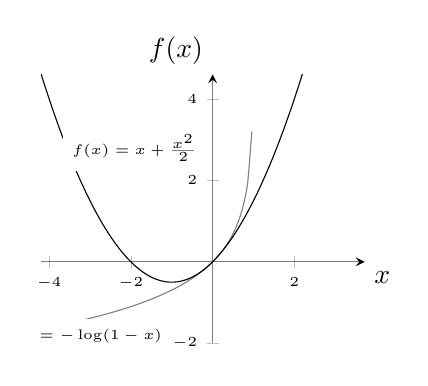
\begin{tikzpicture}
	\begin{axis}[scale=.6,draw opacity =.5,samples=100,smooth, 
	  axis x line=center,
	  axis y line=center,
	  ylabel = {$f(x)$},
	  xlabel = {$x$},
	  xlabel style={below right},
	  ylabel style={above left},
	  xmin=-4.2,xmax=3,ymin=-2,ymax=4,
	  enlargelimits=upper,
	  x tick label style={font=\tiny},
	  y tick label style={font=\tiny}
	  ]
	  \addplot[gray,opacity=1] {-ln(1-x)};
	  \addplot[black,opacity=1] {x+((x^2)/2)};
	  
	  % Etiquetas de las funciones
	  \node[fill=white, anchor=north east] at (axis cs:-1,-1.4) {\tiny$f(x) = -\log(1-x)$};
	  \node[fill=white, anchor=south] at (axis cs:-1.9,2.22) {\tiny$f(x) = x + \frac{x^2}{2}$};
	\end{axis}
    \end{tikzpicture}
\end{center}

\vspace{.5cm}

En el teorema siguiente, utilizaremos un polinomio de grado $n-1$ para aproximar $1/(1-u)$, y con ello obtener un polinomio de grado $n$ que aproxime $log(1-x)$.

%--------------------teorema 2.2
\begin{teo}
    Sea $P_n$ el polinomio de grado $n$ dado por
    $$P_n(x)=x+\dfrac{x^2}{2}+\dfrac{x^3}{3}+\cdots+\dfrac{x^n}{n}=\sum_{k=1}^n \dfrac{x^k}{k}.$$
    Entonces, para todo $x<1$ y todo $n\geq 1$, se tiene
    $$-\log(1-x)=P_n(x)+\int_0^x \dfrac{u^n}{1-u}\; du.$$
	Demostración.-\; A partir de la identidad algebraica
	$$1-u^n = (1-u)\left(1+u+u^2+\cdots + u^{n-1}\right),$$
	obtenemos la fórmula
	$$\dfrac{1}{1-u}=1+u+u^2+\cdots + u^{n-1}+\dfrac{u^n}{1-u}.$$
	para $u\neq 1$. Integrándola entre $0$ y $x$, siendo $x<1$, obtenemos 
	$$-\log(1-x)=P_n(x)+E_n(x),$$
	siendo $E_n(x)$ la intergal,
	$$E_n(x)=\int_0^x \dfrac{u^n}{1-u}\; du.$$
\end{teo}

El valor de $E_m(x)$ representa el error cometido al aproximar $-\log(1-x)$ con el polinomio $P_n(x)$. Para utilizar  $-\log(1-x)=P_n(x)+E_n(x),$ necesitamos conocer si el error es positivo o negativo y lo grande que puede ser.

%--------------------teorema 2.4
\begin{teo}
    Si $0<x<1,$ tenemos las desigualdades
    $$\dfrac{x^{n+1}}{n+1}\leq E_n(x)\leq \dfrac{1}{1-x}\dfrac{x^{n+1}}{n+1}.$$
    Si $x<0$, el error $E_n(x)$ tiene el mismo signo que $(-1)^{n+1}$, y se tiene
    $$0<(-1)^{n+1}E_n(x)\leq \dfrac{|x|}{n+1}.$$\\
	Demostración.-\; Supongamos que $0<x<1$. En la integral que define $E_n(x)$ tenemos $0\leq u\leq x,$ con lo que $1-x\leq 1-u\leq 1,$ y por tanto el integrando satisface las desigualdades
	$$u^n \leq \dfrac{u^n}{1-u}\leq \dfrac{u^n}{1-x}$$
	Integrando estas desigualdades, obtenemos
    $$\dfrac{x^{n+1}}{n+1}\leq E_n(x)\leq \dfrac{1}{1-x}\dfrac{x^{n+1}}{n+1}.$$
    Para demostrar $0<(-1)^{n+1}E_n(x)\leq \dfrac{|x|}{n+1}$, supongamos $x<0$ y sea $t=-x=|x|$. De este modo $t>0$ y tenemos
    $$E_n(x)=E_n(-t)=\int_0^{-t} \dfrac{u^n}{1-u}\; du=-\int_0^t\dfrac{-v^n}{1+v}\; dv = (-1)^{n+1}\int_0^t \dfrac{v^n}{1+v}\; dv.$$
    Esto demuestra que $E_n(x)$ tiene el mismo signo que $(-1)^{n+1}$. Asimismo, tenemos 
    $$(-1)^{n+1}E_n(x)=\int_0^t \dfrac{v^n}{1+v}\; dv \leq \int_0^t v"n \; dv = \dfrac{t^{n+1}}{n+1}=\dfrac{|x|^{n+1}}{n+1},$$
    lo cual completa la demostración.
\end{teo}

El teorema que sigue nos da una fórmula muy útil para los cálculo con logaritmos 

%--------------------teorema 2.5
\begin{teo}
    Si $0<x<1$, y si $m\geq 1$, se tiene
    $$\log\dfrac{1+x}{1-x}=2\left(x+\dfrac{x^3}{3}+\cdots + \dfrac{x^{2m-1}}{2m-1}\right)+R_m(x),$$
    en donde el término de error, $R_m(x)$, satisface las desigualdades
    $$\dfrac{x^{2m+1}}{2m+1}< R_m(x)\leq \dfrac{2-x}{1-x}\dfrac{x^{2m+1}}{2m+1}.$$\\
	Demostración.-\; La igualdad $-\log(1-x)=P_n(x)+E_n(x)$ es válida para cualquier $x$ real tal que $x<1$. Si reemplazamos $x$ por $-x$, manteniendo $x>-1$, obtenemos la fórmula
	$$-\log(1+x)=P_n(-x)+E_n(-x)$$
	Si $-1<x<1$, son válida $-\log(1-x)=P_n(x)+E_n(x)$ y $-\log(1+x)=P_n(-x)+E_n(-x)$. Restando estas dos igualdades, obtenemos
	$$\log \dfrac{1+x}{1-x} = P_n(x)-P_n(-x)+E_n(x)-E_n(-x).$$
	En la diferencia $P_n(x)-P_n(-x)$, las potencias pares de $x$ desaparecen y las potencias impares se duplican. Por consiguiente, si $n$ es par, por ejemplo $n=2m$, tenemos
	$$P_{2m}(x)-P_{2m}(-x) = 2\left(x+\dfrac{x^3}{3}+\cdots+\dfrac{x^{2m-1}}{2m-1}\right),$$
	y la igualdad  $\log \dfrac{1+x}{1-x} = P_n(x)-P_n(-x)+E_n(x)-E_n(-x).$ se transforma en
	$$\log \dfrac{1+x}{1-x} = 2\left(x+\dfrac{x^3}{3}+\cdots+\dfrac{x^{2m-1}}{2m-1}\right)+R_m(x),$$
	donde $R_m(x)=E_{2m}(x)-E_{2m}(-x)$. Esta fórmula es válida si $x$ está en el intervalo abierto $-1<x<1$. Mantengamos ahora $x$ en el intervalo $0<x<1$. Entonces la estimación del teorema 6.4 nos da
	$$\dfrac{x^{2m+1}}{2m+1}<R_m(x)<\dfrac{1}{1-x}\dfrac{x^{2m+1}}{2m+1} \qquad \mbox{y}\qquad 0<-E_{2m}(-x)\leq \dfrac{2^{2m+1}}{2m+1},$$
	Sumando estas desigualdades, obtenemos 
	$$\dfrac{x^{2m+1}}{2m+1}< R_m(x)\leq \dfrac{2-x}{1-x}\dfrac{x^{2m+1}}{2m+1},$$ 
	ya que $1+1/(1 - x) = (2 - x)/(1 - x).$
\end{teo}

\section{Ejercicios}
\begin{enumerate}[1.]

    %--------------------1.
    \item Utilizar el teorema 6.5 poniendo $x=\frac{1}{3}$ y $m=5$ para calcular aproximaciones de $\log(2)$. Conservar nueve cifras decimales en los cálculos y obtener las desigualdades $0,6931460<\log 2 < 0.6931476.$\\\\
	Respuesta.-\; Por el teorema 6.5, tenemos
	$$
	\begin{array}{rcl}
	    \log \dfrac{1+x}{1-x} &=& 2\left(x+\dfrac{x^3}{3}+\dfrac{x^5}{5}+\dfrac{x^7}{7}+\dfrac{x^9}{9}\right)+R_5(x)\\\\
	    \log \dfrac{1+\frac{1}{3}}{1-\frac{1}{3}} &=& 2\left[\dfrac{1}{3}+\dfrac{\left(\frac{1}{3}\right)^3}{3}+\dfrac{\left(\frac{1}{3}\right)^5}{5}+\dfrac{\left(\frac{1}{3}\right)^7}{7}+\dfrac{\left(\frac{1}{3}\right)^9}{9}\right]+R_5\left(\dfrac{1}{3}\right)\\\\
	\end{array}
	$$
	De donde
	$$\dfrac{\left(\frac{1}{3}\right)^9}{9}<R_5\left(\dfrac{1}{3}\right)\leq \left(\dfrac{2-\frac{1}{3}}{1-\frac{1}{3}}\right) \left[\dfrac{\left(\frac{1}{3}\right)^{10}}{10}\right]$$
	Por lo tanto,
	$$0.693146<\log < 0.6931476.$$\\

    %--------------------2.
    \item 

\end{enumerate}
